% !TEX root = QlockToo.tex
% Einstellungen
\documentclass[12pt, a4paper, DIV12, twocolumn]{scrartcl}
\usepackage[utf8]{inputenc}
\usepackage[T1]{fontenc}
\usepackage{lmodern}
\usepackage[ngerman]{babel}
\usepackage{amsmath}
\usepackage{nicefrac}
\usepackage{graphicx, wrapfig, float}
\usepackage[onehalfspacing]{setspace}
\usepackage{paralist}  % \begin{compactitem}
\usepackage{listings, color}
\usepackage[parfill]{parskip}
\usepackage{setspace}
\usepackage{tabularx}
\usepackage{booktabs}
\usepackage{multirow}

\onehalfspacing
\setcounter{tocdepth}{2} % Tiefe Inhaltsverzeichnis
\numberwithin{figure}{section}
\setkomafont{sectioning}{\normalcolor\bfseries}

% -------------------
% Quelltextanzeige
\usepackage{listings, color}

\newcommand{\lstfontfamily}{\ttfamily}
%\newcommand{\lstfontfamily}{\sffamily} % Adapt to schneider
\newcommand{\textlst}[1]{\texttt{#1}}
\newcommand{\mathlst}[1]{\mathtt{#1}}
\lstdefinestyle{tiny}{basicstyle=\tiny\lstfontfamily}
\lstdefinestyle{scriptsize}{basicstyle=\scriptsize\lstfontfamily}
\lstdefinestyle{footnotesize}{basicstyle=\footnotesize\lstfontfamily}
\lstdefinestyle{small}{basicstyle=\small\lstfontfamily}
\lstdefinestyle{normalsize}{basicstyle=\normalsize\lstfontfamily}
\lstdefinestyle{large}{basicstyle=\lstfontfamily}

\lstdefinestyle{monitor}{morekeywords={monitor, export}}
\lstdefinestyle{ConcPascal}{language=Pascal,style=monitor}
\newcommand{\mathcodefont}[1]{\mathtt{#1}}
\newcommand{\codefont}[1]{{\lstfontfamily #1}}
\newlength{\lstframexleftmargin}
\setlength{\lstframexleftmargin}{1mm}

\definecolor{darkviolet}{rgb}{0.5,0,0.4}
\definecolor{darkgreen}{rgb}{0,0.4,0.2}
\definecolor{darkblue}{rgb}{0.1,0.1,0.9}
\definecolor{darkgrey}{rgb}{0.5,0.5,0.5}
\definecolor{lightblue}{rgb}{0.4,0.4,1}

\lstdefinestyle{eclipse}{
    basicstyle=\small\lstfontfamily,
    emphstyle=\color{red}\bfseries,
    keywordstyle=\color{darkviolet}\bfseries,
    commentstyle=\color{darkgreen},
    stringstyle=\color{darkblue},
    numberstyle=\color{darkgrey}\lstfontfamily,
    emphstyle=\color{red},
    % get also javadoc style comments
    morecomment=[s][\color{lightblue}]{/**}{*/},
    morekeywords={@start, @stop, @v, @about, @demo_translation, @demo_forward, @demo_sideways, @demo_stopWithDelay, uint8_t, uint16_t, int16_t, int8_t, byte},
   %columns=fullflexible, %spaceflexible, %flexible, fullflexible
%  escapeinside=`',
%  escapechar=@,
  showstringspaces=false,
  numbers=left
}

\definecolor{lstBg}{rgb}{0.98, 0.98, 0.98}
\definecolor{lstFrame}{rgb}{0.8, 0.8, 0.8}
\lstset{
    language = C,
    style=eclipse,
    tabsize=4,
    basicstyle = \ttfamily,
    title=\lstname,
    % numbers=none,
    backgroundcolor=\color{lstBg},
    rulecolor=\color{lstFrame},
    frame=lines,
    %captionpos=b,
    aboveskip=1\bigskipamount,%{1.5\baselineskip},
    showstringspaces=false,
    extendedchars=true,
    breaklines=false,
    literate=%
        {Ö}{{\"O}}1
        {Ä}{{\"A}}1
        {Ü}{{\"U}}1
        {ß}{{\ss}}1
        {ü}{{\"u}}1
        {ä}{{\"a}}1
        {ö}{{\"o}}1
}


\titlehead{
    \begin{tabular}{l  p{9cm} c}
        & &  
\includegraphics[width=0.4\textwidth]{Abbildungen/W-HS} \\
       & & \textbf{ Fachbereich Maschinenbau }\\

    \end{tabular}
   % Westfälische Hochschule\\Fachbereich Maschinenbau
    \vspace{1.5cm}}

\subject{Projektstudie}

\title{Entwicklung und Fertigung einer elektronischen Wanduhr mit LED-Matrix\vspace{1.5cm}}

\subtitle{Development and implementation of an electronic clock. (We can build a clock, too)\vspace{1.5cm}}

\author{
    \begin{tabular}{rl}
        Manuel Fehmer & 200923513 \\
        Thomas Feldmann & 200923381 \\
        Marlene Feldmann & 200825051 \\
        Carsten Hußmann & 200824460\\
    \end{tabular}\vspace{0.3cm}}

\begin{document}
\begin{titlepage}
\maketitle
\pagenumbering{gobble}
\end{titlepage}
\twocolumn[
   \begin{@twocolumnfalse}
     \tableofcontents
    \end{@twocolumnfalse}
]
\pagenumbering{arabic}
\newpage

% !TEX root = QlockToo.tex
% Kapitelvorlage

\section{Einleitung}
\label{sec:Einleitung}

\begin{figure}[t]
    \centering
    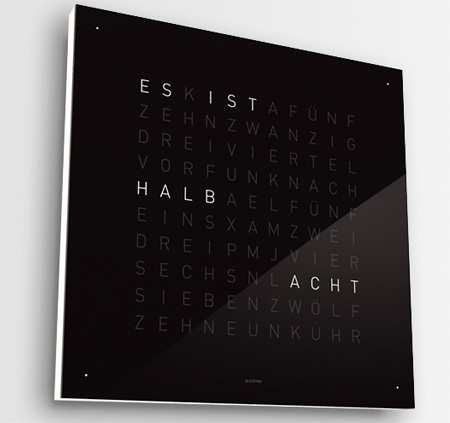
\includegraphics[width=9cm]{Abbildungen/qlocktwo-wand}
    \caption[ClockTwo]{CLOCKTWO CLASSIC}
    \label{fig:ClockTwo}
\end{figure}
%
 \begin{multicols}{2}
 In der heutigen Zeit steht neben der Funktionalität vieler Dinge ihr Design im Vordergrund. Bestes Beispiel ist die CLOCKTWO® der Biegert~\&~Funk Manufacture GmbH \& Co. KG\footnote{\cite{Bie 13}}. Abbildung~\ref{fig:ClockTwo} zeigt die CLOCKTWO CLASSIC als Wand- oder Standuhr. %Die QLOCKTWO® ist ein international eingetragenes Markenzeichen, welches zudem durch internationale Patente und Designpatente geschützt ist. 
 Zeit in zeitlosem Design, so bewirbt die Designmanufaktur die einzigartige Uhr.  Inspiriert durch diese außergewöhnliche Darstellung der Zeit in geschriebenen Worten, entsteht das Entwicklungs- und Fertigungskonzept einer elektronischen Wanduhr mit einer LED-Matrix. \textit{We can built a CLOCK, TOO.}
 \end{multicols}
 %
 \begin{figure}[h]
    \centering
    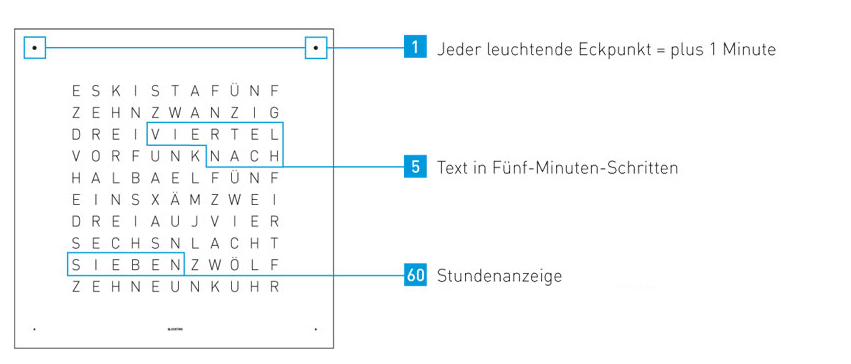
\includegraphics[width=13cm]{Abbildungen/Uhrzeit_Beispiel}
    \caption[Uhrzeit_Bspl]{Beispiel: 7 Uhr 17}
    \label{fig:Uhrzeit_Bspl}
\end{figure}
 %
 \begin{figure}[t]
    \centering
    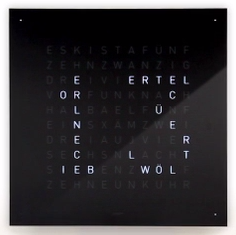
\includegraphics[width=7cm]{Abbildungen/Sekunden}
    \caption[Sekunden]{Darstellung der Sekunden}
    \label{fig:Sekunden}
\end{figure}
%
  \begin{multicols}{2}
Die Zeitanzeige erfolgt auf einer Buchstabenmatrix in Fünf-Minuten-Schritten, siehe Abbildung~\ref{fig:Uhrzeit_Bspl}. Die Worte werden durch Ausleuchten einer Buchstabenfolie auf einer Plexiglasscheibe durch LEDs abgebildet. Durch vier zusätzliche Leuchtpunkte in den Ecken der Uhr werden die Minuten zwischen den Intervallen angezeigt. Abbildung~\ref{fig:Sekunden} zeigt die Darstellung der Sekunden. Auf der kompletten Matrix kann ebenfalls die Raumtemperatur angezeigt werden. Die Umstellung erfolgt sowie die Auswahl weiterer Funktionen über seitliche Taster. Vor der Konzeption der Wortuhr steht die Programmierung einer Desktop-Software, welche den Testprozess der Algorithmen beschleunigt. Die Software ermöglicht zudem die Darstellung weiterer Unterprogramme. 
Bei der Konstruktion sowie die Fertigung des Uhrgehäuses werden Kaufteile mit Eigenproduktionen kombiniert, um dem äußeren Erscheinungsbild des Originals möglichst nah zu kommen und die Kosten gering zu halten. Die Entwicklung eines Elektronikkonzeptes ist  weiterer fundamentaler Bestandteil des Projektes.
\end{multicols}




% !TEX root = QlockToo.tex
% Software
\section{Software}
\label{sec:Software}

\begin{figure}[t]
    \centering
    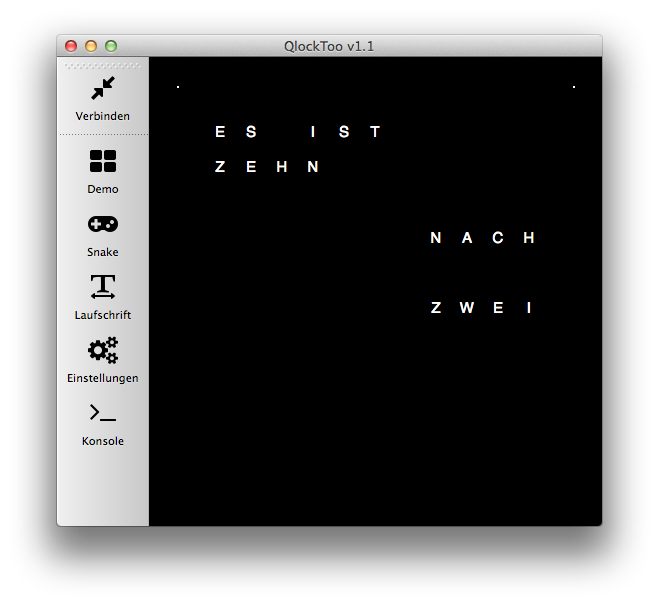
\includegraphics[width=.8\textwidth]{Abbildungen/Software/Hauptfenster}
    \caption[QlockToo-Manager]{Der QlockToo-Manager}
    \label{fig:Manager}
\end{figure}

\begin{multicols}{2}
Im ersten Projektschritt zur Entwicklung der Uhr wird eine Desktop-Software, der QlockToo-Manager, programmiert, welche den Testprozess der Algorithmen deutlich beschleunigt. Mit weiterem Projektfortschritt wächst auch der Programmumfang. Durch stetige Weiterentwicklung kommen zahlreiche Funktionen hinzu, welche im folgenden dargestellt sind:

\begin{itemize}
\item Die Software enthält einen Simulator. Dieser stellt alle Muster und Algorithmen direkt ohne Anschluss an die Hardware dar.
\item Zu Testzwecken sind verschiedene Demonstrationsmuster implementiert.
\item Mit Hilfe einer Laufschrift können frei wählbare Texte angezeigt werden.
\item Das Handyspiel Snake kann auf dem Uhrenschirm gespielt werden. Die Steuerung erfolgt über die Pfeiltasten am Computer.
\item Über eine USB-Schnittstelle fungiert die QlockToo als Display der Software. Das notwendige Streaming-Protokoll wird eigens für diese Anwendung entwickelt.
\item Zur Einstellung der QlockToo über den Computer ist ein Einstellungsdialog implementiert. Dieser ermöglicht zusätzliche Einstellmöglichkeiten über die Funktionen der vier Tasten hinaus.
\end{itemize}

\textbf{Aufbau}
Um eine Lauffähigkeit auf allen gängigen Plattformen (Windows / Mac OS X / Linux) zu realisieren wird die Programmiersprache Python verwendet. Weiterer Vorteil ist die hohe Entwicklungsgeschwindigkeit.
Das aus der C++ - Welt bekannte Framework Qt wird über die von Digia bereitgestellten PySide-Bindings als GUI-Framework genutzt. Die Software baut somit ausschließlich auf freier Open-Source Software auf.

\textbf{Simulator}
Der QlockToo-Manager zeigt nach dem Start den Simulator. Seitlich wird eine Menüleiste zum Starten der Unterprogramme dargestellt.
Solange kein Unterprogramm ausgewählt ist, wird standardmäßig das Programm \emph{Timewords}, welches für die Anzeige der Zeit in Worten zuständig ist, angezeigt. Der QlockToo-Manager bedient sich dazu der momentanen Systemzeit.
Die Unterprogramme sind jeweils einzelne, voneinander unabhängige Python-Module. Eine Erweiterung ist somit jederzeit möglich.
Der Simulator besitzt die gleiche API wie die Hardware. Die Ausgabe der Programme kann somit ohne Anpassungen auf die Hardware gestreamt oder im Simulator angezeigt werden. Auch eine parallele Darstellung ist möglich.
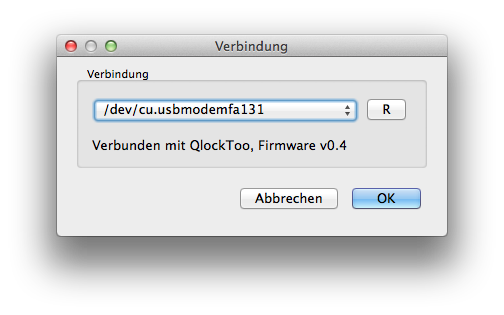
\includegraphics[width=\columnwidth]{Abbildungen/Software/ConnectDialog}
Im Entwicklungsmodus ist eine Konsole integriert, mit der direkt Befehle an die API der QlockToo gesendet werden können. Kommandos und Rückgabewerte werden zur einfacheren optischen Erfassung farblich hervorgehoben.
{
    \centering
    \includegraphics[width=0.9\columnwidth]{Abbildungen/Software/Linux}
}

\textbf{Demonstrationsmuster}
Der zweite Punkt in der Menüleiste sind die Demonstrationsmuster. Zur besseren Sichtbarkeit sind die Muster invertiert dargestellt. Folgende Demonstrationen stehen zur Verfügung:

\textbf{Pulse}
Alle LEDs wechseln sanft zwischen minimaler und maximaler Helligkeit.

\textbf{Fade}
Ein Helligkeitsverlauf bewegt sich sinusförmig von links nach rechts und zurück.
{
    \centering
    
\includegraphics[width=\columnwidth]{Abbildungen/Software/Demo/Fade}
}

\textbf{Pixeltest}
Alle Pixel bzw. Buchstaben werden einzeln nacheinander beleuchtet. Diese Demo dient hauptsächlich der Überprüfung der Verkabelung.

\textbf{Wave}
Das Muster Wave zeigt ein pulsierendes Wellenbild, dessen Zentrum mit der Zeit langsam über den Bildschirm wandert.
{
    \centering
    
\includegraphics[width=\columnwidth]{Abbildungen/Software/Demo/Welle}
}

\textbf{Helix}
Die Helix-Darstellung zeigt die zweidimensionale Projektion einer dreidimensionalen Spirale. Die z-Achse wird dabei über unterschiedliche Helligkeitswerte visualisiert. Bedingt durch die Berechnung der Funktionswerte für diskrete Buchstaben auf der Uhr und die geringe Pixelanzahl (110) wirkt die Demonstration zunächst sehr dünn und zerstückelt. Durch die Implementierung eines Gauss-Tiefpasses, wird der gewünschte Anti-Alias-Effekt erzielt. Der 3D~Effekt der Darstellung ist somit sehr viel deutlicher.
{
    \centering
    
\includegraphics[width=\columnwidth]{Abbildungen/Software/Demo/Helix}
}

\textbf{Game Of Life}
Darstellung von Conways Game of Life\footnote{[Con 13]}, anhand toter (schwarz) und lebender (weiß) Zellen.
{
    \centering
    
\includegraphics[width=\columnwidth]{Abbildungen/Software/Demo/Helix}
}

Grundlage sind die vier folgenden Regeln, die bei jeder Iteration abgefragt werden:
\begin{itemize}
    \item Eine tote Zelle mit genau drei lebenden Nachbarn wird in der Folgegeneration neu geboren.
    \item Lebende Zellen mit weniger als zwei lebenden Nachbarn sterben in der Folgegeneration an Einsamkeit.
    \item Eine lebende Zelle mit zwei oder drei lebenden Nachbarn bleibt in der Folgegeneration lebend.
    \item Lebende Zellen mit mehr als drei lebenden Nachbarn sterben in der Folgegeneration an Überbevölkerung.
\end{itemize}

\textbf{Matrix}
Der berühmte Animationseffekt aus dem Film \emph{Matrix} bietet sich aufgrund des Designs der QlockToo besonders an.
{
    \centering
    
\includegraphics[width=\columnwidth]{Abbildungen/Software/Demo/Matrix}
}

\textbf{Laufschrift}
Der vierte Punkt in der Menüleiste ist die Laufschrift. Über ein Fenster kann ein beliebiger Text eingegeben werden, welcher auf der Uhr als Laufschrift abgespielt werden soll. Zum Abspielen muss ein Häkchen im entsprechenden Kontrollkästchen gesetzt werden.
{
    \centering
    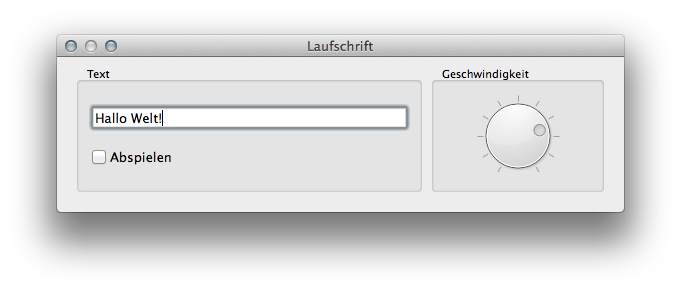
\includegraphics[width=1\columnwidth]{Abbildungen/Software/Laufschrift}
}
Ohne das Häkchen werden bei der Eingabe die einzelnen Buchstaben angezeigt. Über den Drehregler können die Laufrichtung und die Geschwindigkeit variiert werden.

\end{multicols}

% !TEX root = QlockToo.tex
% Firmware

\begin{figure}
    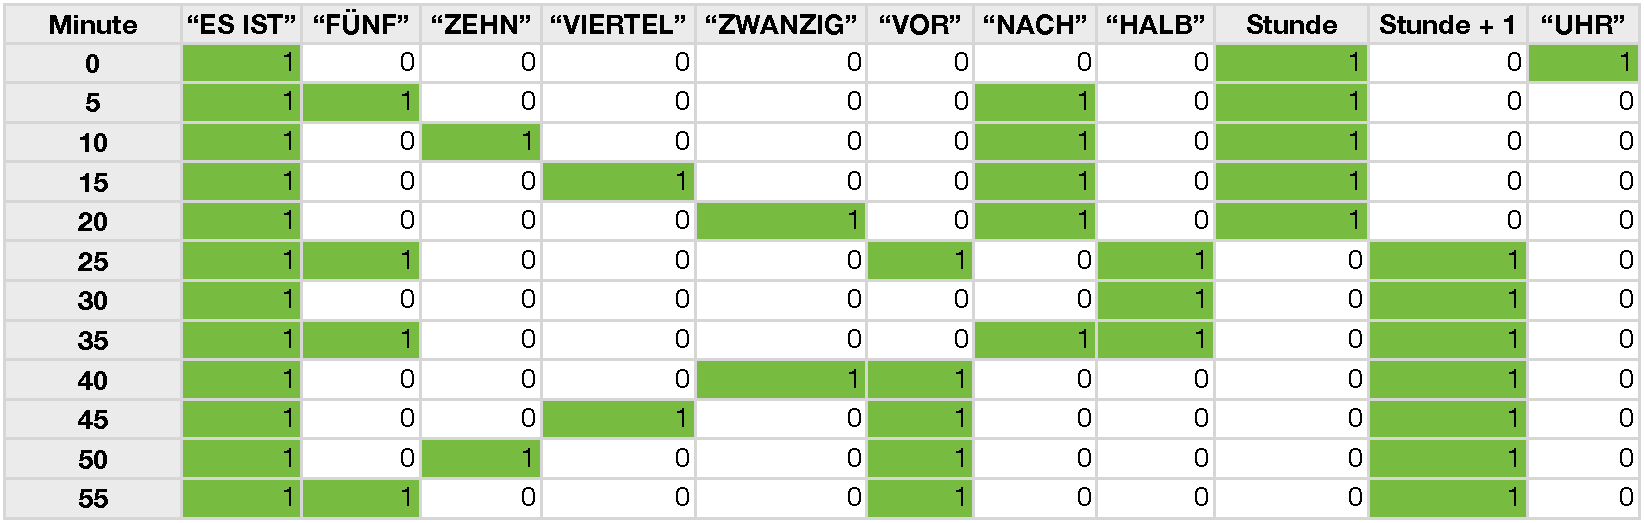
\includegraphics[width=\columnwidth]{Abbildungen/Firmware/Logik}
   
\end{figure}

\section{Firmware}
\label{sec:Firmware}
Die Firmware der QlockToo ist in \emph{C} geschrieben und nutzt Funktionen des Arduino-Cores.
Im Folgenden werden die einzelnen Module der Firmware kurz erläutert.

\begin{multicols}{2}
\textbf{Firmware}
Die Hauptdatei der Firmware enthält den Einstiegspunkt in das Programm und initialisiert alle Module. Hier wird der Haupttimer (1kHz) gestartet, der Displayanzeige und Steuerungsfunktionen übernimmt.

\textbf{Display}
Im Display-Modul wird die Verbindung mit dem I2C-LED-Treiber hergestellt und die Ports für die Ansteuerung der Leistungstransistoren werden konfiguriert.

In der Display-Update-Routine findet das eigentliche Multiplexing statt. Es wird jeweils die nächste LED-Reihe eingeschaltet und die darzustellenden Spalten über die I2C-Schnittstelle an den LED-Treiber gesendet.
Diese Funktion ist besonders zeitkritisch, da ineffiziente Programmierung hier sofort zu einem flimmernden Bild führt.
Die QlockToo baut das Bild 100 mal pro Sekunde komplett auf (Multiplexing mit 1kHz über zehn Reihen), mit bloßen Auge ist daher kein Flimmern zu erkennen.

\textbf{Controller}
Im Controller-Modul befindet sich ein Zustandsautomat, welcher den Betriebsmodus (Zeitanzeige, Temperaturanzeige, usw.) verwaltet.
Der Betriebsmodus der Uhr kann über die Taster eingestellt werden. Das dazu notwendige Abfragen der Taster findet ebenfalls in diesem Modul statt.

\textbf{Timewords}
In diesem Modul ist die dargestellte Logiktabelle für die Anzeige der Zeit in Sätzen in deutscher Sprache implementiert.
Welche LEDs für die gewählten Wörter und Stunden zu beleuchten sind, wird für jedes Wort in Form eines Integers für die Reihe und einer Bitmaske für die Spalten definiert. \emph{Stunde} und \emph{Stunde + 1} sind Platzhalter für die aktuelle und die nächste Stunde.

\textbf{Api}
Die QlockToo kommuniziert per USB über das UART-Protokoll bei 115200 baud mit der Software.
Zum Parsen der empfangenen Befehle wird auf Seite der Firmware die Library \emph{SerialCommand}\footnote{https://github.com/kroimon/Arduino-SerialCommand} eingesetzt.

\textbf{Brightness}
Das Modul Brightness beinhaltet die Steuerung der Helligkeit der QlockToo. Neben dem Automatikmodus, welcher die Helligkeit der Abhängigkeit von den gemessenen Werten des Helligkeitssensors steuert, besteht die Möglichkeit einer manuellen Steuerung. Dabei stehen verschiedene Abstufungen zur Verfügung.

\textbf{DCF77}
In diesem Modul ist der Parser für das DCF77 Signal implementiert. Das DCF77-Signal ist zeitkritisch und wird daher in Interrupts bearbeitet.
Sobald alle notwendigen Daten vorhanden sind -- was mindestens eine Minute dauert -- und der Paritätscheck erfolgreich ist, wird die globale interne Uhrzeit eingestellt.

\textbf{Matrix}
Im Modul \emph{Matrix} sind Funktionen zu Manipulation der Anzeigematrix zusammengefasst. Diese reichen vom Leeren und Füllen der Matrix hin zum Anzeigen von Zahlen und Buchstaben. Die Schriftarten sind in der Datei \emph{font.h} hinterlegt.

\textbf{Thermo}
Dieses Modul enthält die Umrechnung der gemessenen Spannung am Thermistor in eine Temperatur in Celsius.
Dazu kommen Anzeigefunktionen, die die Temperatur auf dem Display ausgeben.
Für die Anzeige der Temperatur wird eine kleinere Schriftart (3x5) genutzt als für die Anzeige der Sekunden (5x7), da noch das Gradzeichen angezeigt wird.

\textbf{Time}
Die QlockToo nutzt den internen 16-Bit Timer1 dazu, die Zeit einzuhalten.
Der Timer wird mit einem Prescaler von 256 Overflow-Betrieb genutzt und mit dem Wert 3036 vorgeladen.
Dadurch feuert der Timer exakt sekündlich und zählt Minuten und Stunden hoch.

\end{multicols}

% !TEX root = QlockToo.tex
\begin{multicols}{2}
\section{Elektronik}
\label{sec:Elektronik}
Während sich Konstruktion und Basisfunktionen der Worduhr sehr eng am Original orientieren, ist die Umsetzung in der Elektronik komplett selbst entwickelt.

\textbf{LED-Matrix} Die LED-Matrix mit 10~x~11 Pixel wird von einem Mikrocontroller angesteuert. Dies geschieht zeilenweise im Multiplexing-Verfahren. Hierbei wird die erste Zeile von einem Transistor mit Spannung versorgt. Die 11 Pixel der Zeile werden über einen LED-Treiber simultan angesteuert. Nach einer Millisekunde wird die Zeile ausgeschaltet, es werden neue Daten in den LED-Treiber geschrieben und die nächste Zeile wird eingeschaltet. 

\textbf{Arduino Mirco}

Als Mikrocontroller wird ein Arduino Micro Board mit dem Atmel Atmega 32U4 Controller verwendet. Der Einsatz eines Arduino Boards vereinfacht die Umsetzung einer seriellen Schnittstelle und verringert durch das bereits vielfach genutzte Board die Fehlerquellen im Layout. Durch die kleine Bauform und die sich aus den Features ergebenden Anforderungen (serielle Kommunikation, $I^{2}C$-Bus, externer Interrupt, 4x Digital Input, 2x Analogeingang und 10x Digital Output) fiel die Auswahl auf den Arduino Micro.

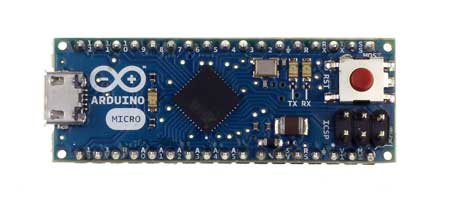
\includegraphics[width=\columnwidth]{Abbildungen/Elektronik/ArduinoMicro}

\textbf{LED-Treiber}

Der TLC59116 LED-Treiber von Texas Instruments hat 16 PWM-Ausgänge mit 8Bit Auflösung - 255 Helligkeitsstufen - und eine Stromregelung, die es ermöglicht auf Vorwiderstände an den LED zu verzichten. Der IC wird über $I^{2}C$ angesteuert. Die Adresse kann hardwareseitig in den letzten 4Bit eingestellt werden und ist auf der Platine hart mit 0b1100 000[R/W] adressiert. Der LED-Treiber ist in der SMD TSSOP-28 Bauform.

\textbf{Transistoren}


\textbf{Transistoren} Die Zeilen werden mit IRF7416 P-FET-Transistoren geschaltet und mit $5V$ versorgt. Die Transistoren werden mit einem Pull-Up Widerstand am Gate beschaltet und mit einem invertierten Signal angesteuert (4~-~13). Die Transistoren haben S0-8 Gehäusebauform. 

\textbf{Taster} Die vier Kurzhubtaster an der rechten Rahmenseite befinden sich auf einer eigenen Platine mit Verbindungskabel. Zur Entprellung befindet sich kurz vor den vier IO-Pins (A2~-~A5) des Controllers ein RC-Glied. 

{
\centering 
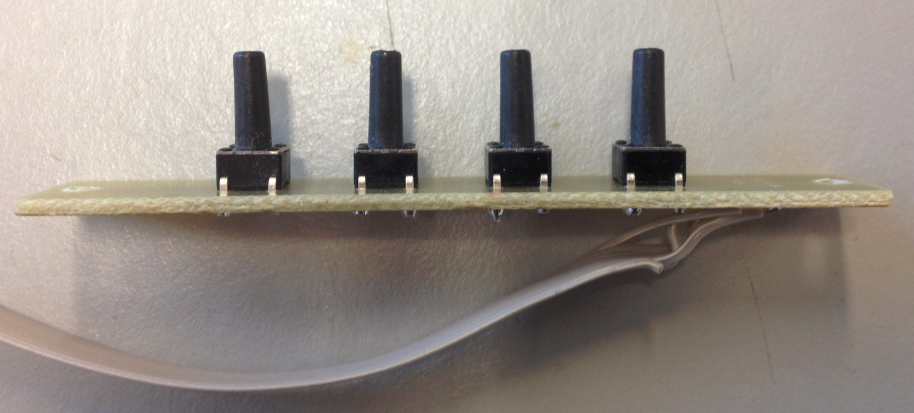
\includegraphics[width=0.9\columnwidth]{Abbildungen/Konstruktion/Taster02} 

}

{
\centering 

\includegraphics[width=0.8\columnwidth]{Abbildungen/Elektronik/Taster01} 

}

Die vier Kurzhubtaster an der rechten Rahmenseite befinden sich auf einer eigenen Platine mit Verbindungskabel. Zur Entprellung befindet sich kurz vor den vier IO-Pins (A2~-~A5) des Controllers ein RC-Glied. 

\textbf{Sensoren}

Als Helligkeitssensor wird ein LDR und als Temperatursensor ein NTC verwendet, in beiden Fällen über Steckverbindung verbunden und einem Trimmpoti als Spannungsteiler an einem Analogeingang (A0~-~A1) des Mikrocontrollers. Der Helligkeitssensor befindet sich mittig oberhalb der Buchstabenmatrix hinter einem Loch in der Folie. Der Temperatursensor befindet sich seitlich am Rahmen um den Einfluss der möglichen Erwärmung der Elektronik auf den Sensor zu verringern. \newline
{
\centering 
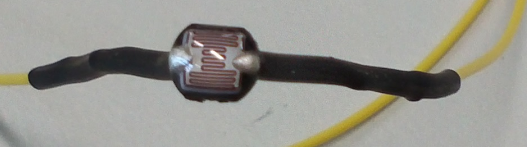
\includegraphics[width=0.9\columnwidth]{Abbildungen/Elektronik/LDR} 

}

{
\centering
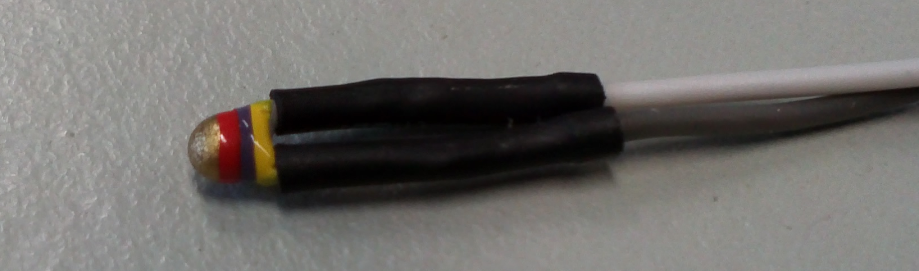
\includegraphics[width=0.9\columnwidth]{Abbildungen/Elektronik/NTC} 

}

\textbf{DCF77} Das DCF77-Modul empfängt das Mitteleuropäische Zeitsignal und verstärkt es. Um das Signal problemlos zu Empfangen wird hier ein interruptfähiger Eingang des Mikrocontrollers (1) verwendet. Durch regelmäßigen Empfang des DCF77 Zeitsignals ist die Genauigkeit des verbauten Quarz hinreichend genau.\newline

\textbf{Spannungsversorgung} Die Spannungsversorgung ist auf den Betrieb mit einem Gleichspannungsnetzteil (7~-~18$V$) ausgelegt und in die zwei Bereiche Elektronik und LED aufgeteilt. Der Bereich Elektronik wird von dem Spannungsregler auf dem Arduino Board versorgt. Die LEDs haben einen eigenen LM7805 Spannungsregler mit 1,5A Ausgangsstrom. An der Hohlsteckerbuchse am Rahmen kann alternativ ein Brückengleichrichter eingelötet werden, dieser verhindert die Verpolung des Netzteils und reduziert den Spannungsfall an den Spannungsreglern. Im Normalbetrieb benötigt die QlockToo 0,1A und 0,23A bei voller Helligkeit aller LED. 

\end{multicols}

{
\centering 
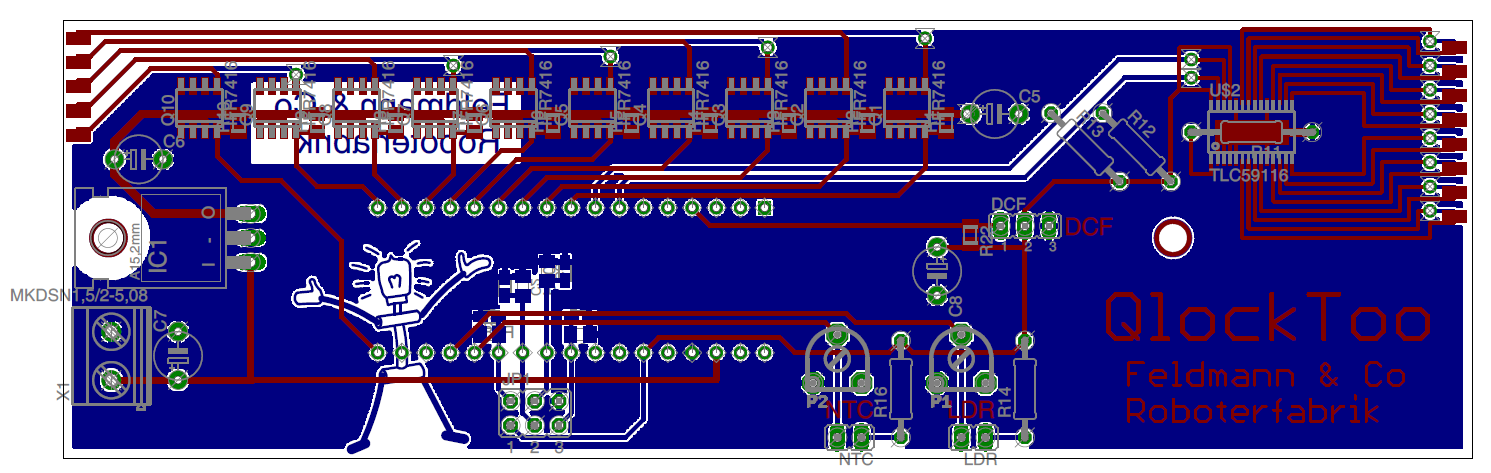
\includegraphics[width=\textwidth]{Abbildungen/Elektronik/Layout01} 
}
\begin{multicols}{2}

\textbf{Platinenlayout}

Das Platinenlayout wurde mit dem PCB Design Tool CADSoft Eagle erstellt. Die Leiterbahnen des Top-Layers sind in Rot dargestellt und die Leiterbahnen, sowie die Massefläche, des Bottom-Layers sind in Blau dargestellt. Im oberen Bereich des Top-Layers befinden sich die 10 P-FET Transistoren mit  Pull-Up Widerständen. Rechts befindet sich der LED-Treiber mit dem Widerstand zur Stromregelung auf der Platinenunterseite. Links befindet sich der LM7805 und darunter der Spannungsanschluss. Mittig auf der Platine sind die Buchsenleisten für den Arduino Micro und das DCF77-Modul. Unten sind die Stiftleisten für den Stecker zum Tasterboard und die Spannungsteiler für NTC und LDR. Unterhalb des Arduino sind die RC-Glieder der Taster angeordnet. Desweiteren verläuft der $I^{2}C$-Bus mit den Pull-Up Widerständen auf dem Bottom-Layer durch die Massefläche. Auf Grund der eigenen Platinenfertigung und dem Verzicht von Durchkontaktierungen müssen einige Bauteile auf beiden Platinenseiten eingelötet werden und die nötigen Durchkontaktierungen mit Draht erstellt werden. Die Stiftleisten für den 10-poligen und den 16-poligen Stecker zur LED-Matrix werden stirnseitig angelötet. 


Die Platine wird aus einer zweiseitigen Fotoplatine erstellt. Hierzu werden Top- und Bottom-Film auf der Fotoplatine ausgerichtet und die Platine drei Minuten mit UV-Licht belichtet. Im Entwicklerbad mit Natriumhydroxid wird der belichtete Fotolack abgewaschen. Die belichteten Stellen auf der Platine werden in einer Ätzanlage mit Eisentrichlorid entfernt. Je nach Güte des Ätzmittels verbleiben nach bereits zwei Minuten im Ätzbad nur noch die unter dem unbelichteten Fotolack liegenden Leiterbahnen. Im Nachgang wird die geätzte Platine nochmals vollständig belichtet, der Fotolack im Entwicklerbad abgewaschen und die Platine mit Kunststofflack beschichtet.

\textbf{Anschluss} Der Arduino Micro wird mit zwei Buchsenleisten\footnote{USB-Stecker in Richtung Spannungsregler} auf die Platine aufgesteckt und bildet mit seinem ISP-Stecker das höchste Bauteil. Die Flachbandkabelstecker zur LED-Matrix werden mit der Nase nach oben aufgesteckt. Die Taster werden mit der Nase des sechspoligen Steckers in Richtung Matrix angeschlossen. Das DCF-Modul wird mit einem dreipoligen gewinkelten Stecker mit Winkel in Richtung Matrix angeschlossen. LDR und NTC besitzen keine Polarität, hierbei ist die Anschlussrichtung egal.
\end{multicols}
{
\centering 
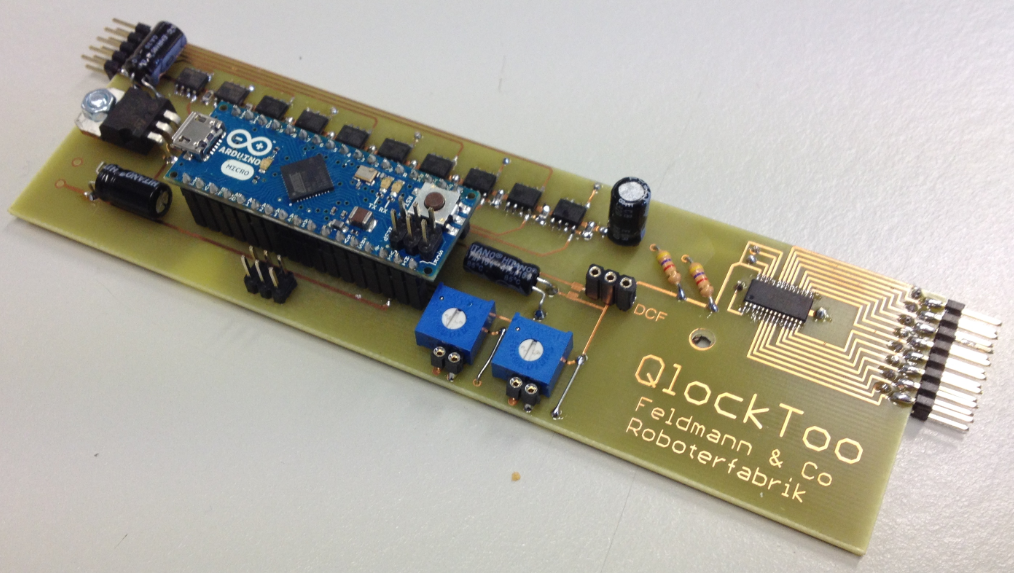
\includegraphics[width=\textwidth]{Abbildungen/Elektronik/Platine_bestueckt} 
}


\begin{landscape}
	\begin{figure}[H]
		\centering
		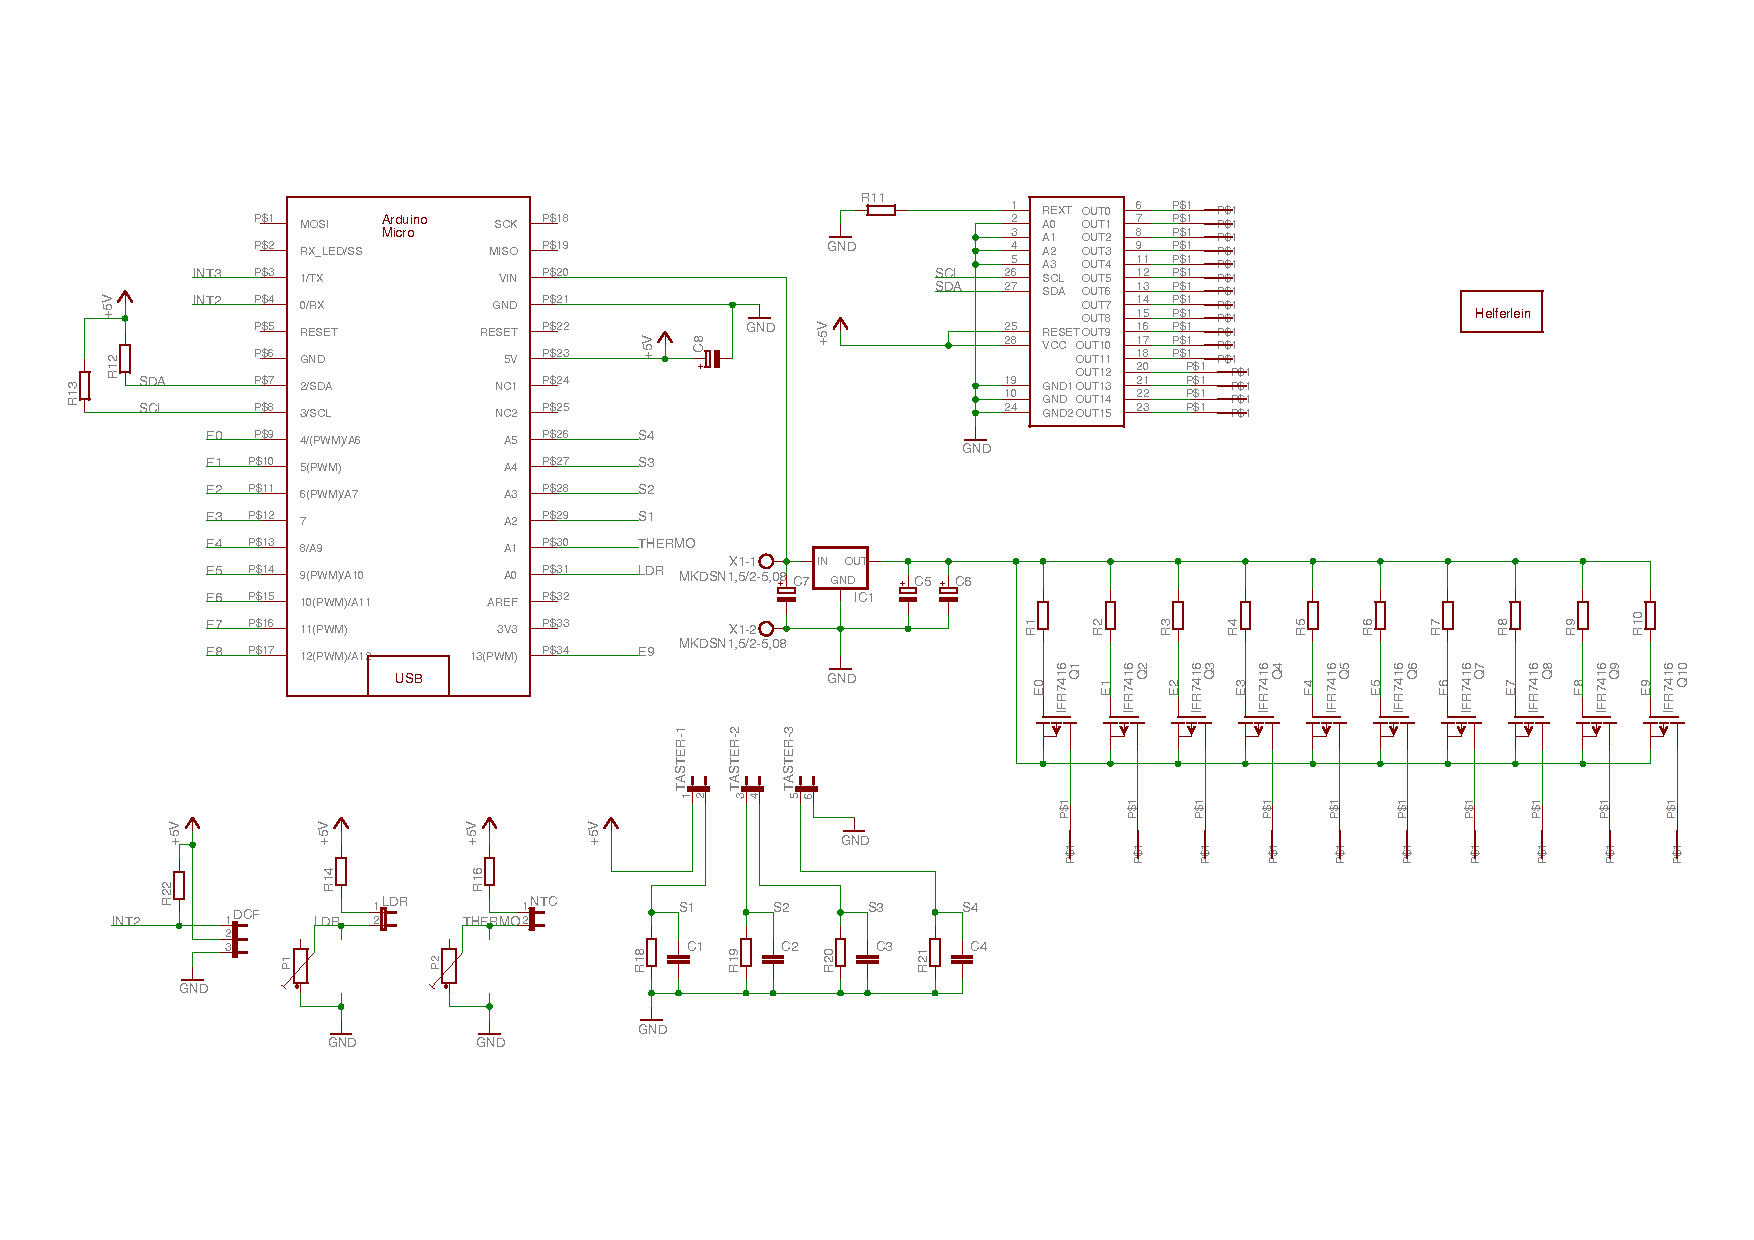
\includegraphics[width=22cm]{Abbildungen/QlockToo_Schaltplan}
		
	\end{figure}
\end{landscape}


\end{document}
